\documentclass[border=4mm]{standalone}
\usepackage[utf8]{inputenc}
\usepackage[T1]{fontenc}
\usepackage{lmodern}
\usepackage{xcolor}
\usepackage{tikz}
\usetikzlibrary{shapes.geometric, arrows.meta, positioning, calc, fit, backgrounds}

% Curated Modern Academic Palette
\definecolor{stage1border}{HTML}{2563EB} % Blue
\definecolor{stage1header}{HTML}{1D4ED8}
\definecolor{stage1bg}{HTML}{F8FAFC}

\definecolor{stage2border}{HTML}{059669} % Emerald
\definecolor{stage2header}{HTML}{047857}
\definecolor{stage2bg}{HTML}{F8FAFC}

\definecolor{stage3border}{HTML}{D97706} % Amber
\definecolor{stage3header}{HTML}{B45309}
\definecolor{stage3bg}{HTML}{F8FAFC}

\definecolor{stage4border}{HTML}{7C3AED} % Purple
\definecolor{stage4header}{HTML}{6D28D9}
\definecolor{stage4bg}{HTML}{F8FAFC}

\definecolor{cardborder}{HTML}{CBD5E1}
\definecolor{textdark}{HTML}{0F172A}
\definecolor{textgray}{HTML}{334155}
\definecolor{codecol}{HTML}{0284C7}
\definecolor{arrowcol}{HTML}{64748B}

\begin{document}
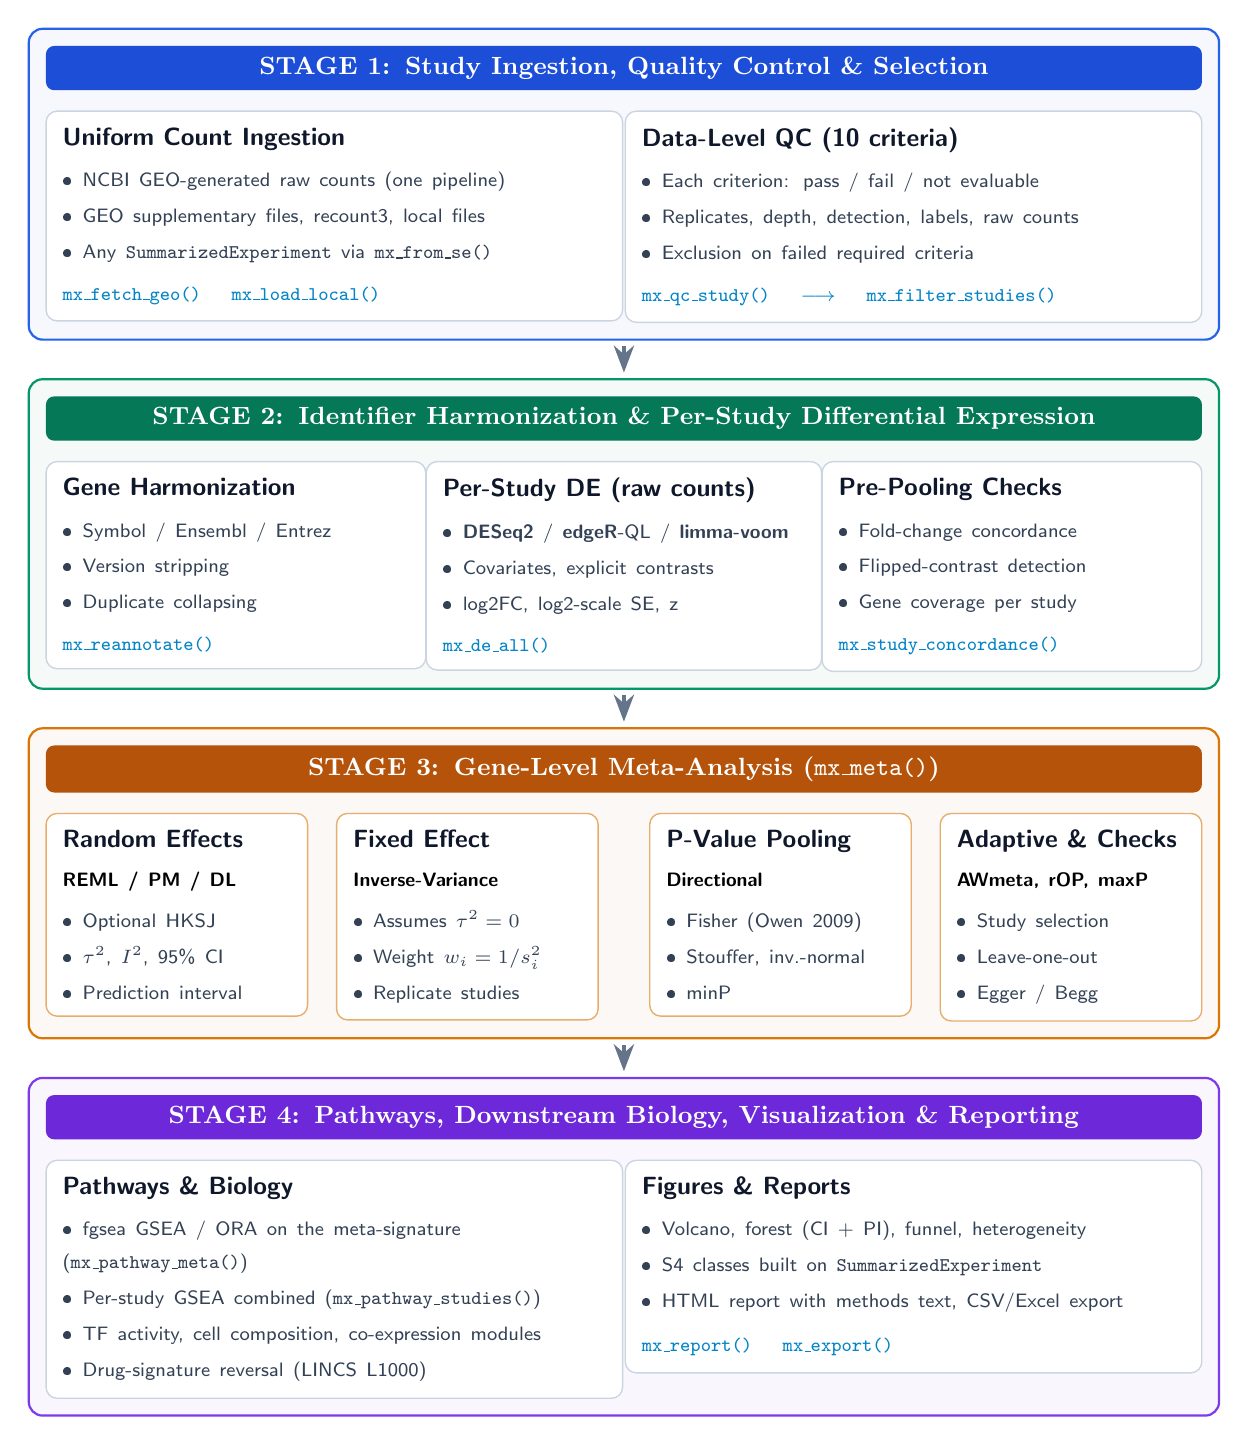
\begin{tikzpicture}[
    font=\sffamily,
    >=Stealth,
    headerbar/.style={
        rectangle,
        rounded corners=3pt,
        text=white,
        font=\small\bfseries,
        inner sep=4pt,
        text width=14.4cm,
        align=center
    },
    innercard/.style={
        rectangle,
        fill=white,
        draw=cardborder,
        line width=0.5pt,
        rounded corners=4pt,
        inner sep=6pt,
        align=left
    },
    flowarrow/.style={
        ->,
        line width=1.5pt,
        draw=arrowcol,
        shorten >=2pt,
        shorten <=2pt
    }
]

% ==============================================================================
% STAGE 1: INGESTION & QC
% ==============================================================================
\node[headerbar, fill=stage1header] (h1) {
    \textbf{STAGE 1: Study Ingestion, Quality Control \& Selection}
};

\node[innercard, text width=6.9cm, minimum height=2.3cm, below=0.25cm of h1.south west, anchor=north west] (c1a) {
    {\small\bfseries\textcolor{textdark}{Uniform Count Ingestion}}\\[3pt]
    {\scriptsize\textcolor{textgray}{• NCBI GEO-generated raw counts (one pipeline)}}\\[1pt]
    {\scriptsize\textcolor{textgray}{• GEO supplementary files, recount3, local files}}\\[1pt]
    {\scriptsize\textcolor{textgray}{• Any \texttt{SummarizedExperiment} via \texttt{mx\_from\_se()}}}\\[3pt]
    {\scriptsize\bfseries\textcolor{codecol}{\texttt{mx\_fetch\_geo()} \quad \texttt{mx\_load\_local()}}}
};

\node[innercard, text width=6.9cm, minimum height=2.3cm, below=0.25cm of h1.south east, anchor=north east] (c1b) {
    {\small\bfseries\textcolor{textdark}{Data-Level QC (10 criteria)}}\\[3pt]
    {\scriptsize\textcolor{textgray}{• Each criterion: pass / fail / not evaluable}}\\[1pt]
    {\scriptsize\textcolor{textgray}{• Replicates, depth, detection, labels, raw counts}}\\[1pt]
    {\scriptsize\textcolor{textgray}{• Exclusion on failed required criteria}}\\[3pt]
    {\scriptsize\bfseries\textcolor{codecol}{\texttt{mx\_qc\_study()} \quad $\longrightarrow$ \quad \texttt{mx\_filter\_studies()}}}
};

\begin{scope}[on background layer]
    \node[rectangle, rounded corners=5pt, fill=stage1header!4, draw=stage1border, line width=0.8pt,
          fit=(h1)(c1a)(c1b), inner sep=6pt] (box1) {};
\end{scope}

% ==============================================================================
% STAGE 2: HARMONIZATION & DIFFERENTIAL EXPRESSION
% ==============================================================================
\node[headerbar, fill=stage2header, below=0.7cm of box1.south] (h2) {
    \textbf{STAGE 2: Identifier Harmonization \& Per-Study Differential Expression}
};

\node[innercard, text width=4.4cm, minimum height=2.3cm, below=0.25cm of h2.south west, anchor=north west] (c2a) {
    {\small\bfseries\textcolor{textdark}{Gene Harmonization}}\\[3pt]
    {\scriptsize\textcolor{textgray}{• Symbol / Ensembl / Entrez}}\\[1pt]
    {\scriptsize\textcolor{textgray}{• Version stripping}}\\[1pt]
    {\scriptsize\textcolor{textgray}{• Duplicate collapsing}}\\[3pt]
    {\scriptsize\bfseries\textcolor{codecol}{\texttt{mx\_reannotate()}}}
};

\node[innercard, text width=4.4cm, minimum height=2.3cm, below=0.25cm of h2.south east, anchor=north east] (c2c) {
    {\small\bfseries\textcolor{textdark}{Pre-Pooling Checks}}\\[3pt]
    {\scriptsize\textcolor{textgray}{• Fold-change concordance}}\\[1pt]
    {\scriptsize\textcolor{textgray}{• Flipped-contrast detection}}\\[1pt]
    {\scriptsize\textcolor{textgray}{• Gene coverage per study}}\\[3pt]
    {\scriptsize\bfseries\textcolor{codecol}{\texttt{mx\_study\_concordance()}}}
};

\node[innercard, text width=4.6cm, minimum height=2.3cm] at ($(c2a.east)!0.5!(c2c.west)$) (c2b) {
    {\small\bfseries\textcolor{textdark}{Per-Study DE (raw counts)}}\\[3pt]
    {\scriptsize\textcolor{textgray}{• \textbf{DESeq2} / \textbf{edgeR}-QL / \textbf{limma-voom}}}\\[1pt]
    {\scriptsize\textcolor{textgray}{• Covariates, explicit contrasts}}\\[1pt]
    {\scriptsize\textcolor{textgray}{• log2FC, log2-scale SE, z}}\\[3pt]
    {\scriptsize\bfseries\textcolor{codecol}{\texttt{mx\_de\_all()}}}
};

\begin{scope}[on background layer]
    \node[rectangle, rounded corners=5pt, fill=stage2header!4, draw=stage2border, line width=0.8pt,
          fit=(h2)(c2a)(c2b)(c2c), inner sep=6pt] (box2) {};
\end{scope}

% ==============================================================================
% STAGE 3: META-ANALYSIS
% ==============================================================================
\node[headerbar, fill=stage3header, below=0.7cm of box2.south] (h3) {
    \textbf{STAGE 3: Gene-Level Meta-Analysis (\texttt{mx\_meta()})}
};

\node[innercard, draw=stage3border!60, text width=2.9cm, minimum height=2.3cm, below=0.25cm of h3.south west, anchor=north west] (e1) {
    {\small\bfseries\textcolor{textdark}{Random Effects}}\\[2pt]
    {\scriptsize\textbf{REML / PM / DL}}\\[3pt]
    {\scriptsize\textcolor{textgray}{• Optional HKSJ}}\\[1pt]
    {\scriptsize\textcolor{textgray}{• $\tau^2$, $I^2$, 95\% CI}}\\[1pt]
    {\scriptsize\textcolor{textgray}{• Prediction interval}}
};

\node[innercard, draw=stage3border!60, text width=2.9cm, minimum height=2.3cm, below=0.25cm of h3.south east, anchor=north east] (e4) {
    {\small\bfseries\textcolor{textdark}{Adaptive \& Checks}}\\[2pt]
    {\scriptsize\textbf{AWmeta, rOP, maxP}}\\[3pt]
    {\scriptsize\textcolor{textgray}{• Study selection}}\\[1pt]
    {\scriptsize\textcolor{textgray}{• Leave-one-out}}\\[1pt]
    {\scriptsize\textcolor{textgray}{• Egger / Begg}}
};

\node[innercard, draw=stage3border!60, text width=2.9cm, minimum height=2.3cm, right=0.35cm of e1.north east, anchor=north west] (e2) {
    {\small\bfseries\textcolor{textdark}{Fixed Effect}}\\[2pt]
    {\scriptsize\textbf{Inverse-Variance}}\\[3pt]
    {\scriptsize\textcolor{textgray}{• Assumes $\tau^2 = 0$}}\\[1pt]
    {\scriptsize\textcolor{textgray}{• Weight $w_i = 1/s_i^2$}}\\[1pt]
    {\scriptsize\textcolor{textgray}{• Replicate studies}}
};

\node[innercard, draw=stage3border!60, text width=2.9cm, minimum height=2.3cm, left=0.35cm of e4.north west, anchor=north east] (e3) {
    {\small\bfseries\textcolor{textdark}{P-Value Pooling}}\\[2pt]
    {\scriptsize\textbf{Directional}}\\[3pt]
    {\scriptsize\textcolor{textgray}{• Fisher (Owen 2009)}}\\[1pt]
    {\scriptsize\textcolor{textgray}{• Stouffer, inv.-normal}}\\[1pt]
    {\scriptsize\textcolor{textgray}{• minP}}
};

\begin{scope}[on background layer]
    \node[rectangle, rounded corners=5pt, fill=stage3header!4, draw=stage3border, line width=0.8pt,
          fit=(h3)(e1)(e2)(e3)(e4), inner sep=6pt] (box3) {};
\end{scope}

% ==============================================================================
% STAGE 4: INTERPRETATION & REPORTING
% ==============================================================================
\node[headerbar, fill=stage4header, below=0.7cm of box3.south] (h4) {
    \textbf{STAGE 4: Pathways, Downstream Biology, Visualization \& Reporting}
};

\node[innercard, text width=6.9cm, minimum height=2.45cm, below=0.25cm of h4.south west, anchor=north west] (c4a) {
    {\small\bfseries\textcolor{textdark}{Pathways \& Biology}}\\[3pt]
    {\scriptsize\textcolor{textgray}{• fgsea GSEA / ORA on the meta-signature (\texttt{mx\_pathway\_meta()})}}\\[1pt]
    {\scriptsize\textcolor{textgray}{• Per-study GSEA combined (\texttt{mx\_pathway\_studies()})}}\\[1pt]
    {\scriptsize\textcolor{textgray}{• TF activity, cell composition, co-expression modules}}\\[1pt]
    {\scriptsize\textcolor{textgray}{• Drug-signature reversal (LINCS L1000)}}
};

\node[innercard, text width=6.9cm, minimum height=2.45cm, below=0.25cm of h4.south east, anchor=north east] (c4b) {
    {\small\bfseries\textcolor{textdark}{Figures \& Reports}}\\[3pt]
    {\scriptsize\textcolor{textgray}{• Volcano, forest (CI + PI), funnel, heterogeneity}}\\[1pt]
    {\scriptsize\textcolor{textgray}{• S4 classes built on \texttt{SummarizedExperiment}}}\\[1pt]
    {\scriptsize\textcolor{textgray}{• HTML report with methods text, CSV/Excel export}}\\[4pt]
    {\scriptsize\bfseries\textcolor{codecol}{\texttt{mx\_report()} \quad \texttt{mx\_export()}}}
};

\begin{scope}[on background layer]
    \node[rectangle, rounded corners=5pt, fill=stage4header!4, draw=stage4border, line width=0.8pt,
          fit=(h4)(c4a)(c4b), inner sep=6pt] (box4) {};
\end{scope}

% ==============================================================================
% CLEAN VERTICAL CONNECTING ARROWS BETWEEN STAGES
% ==============================================================================
\draw[flowarrow] (box1.south) -- (box2.north);
\draw[flowarrow] (box2.south) -- (box3.north);
\draw[flowarrow] (box3.south) -- (box4.north);

\end{tikzpicture}
\end{document}
